\documentclass{article}\usepackage[]{graphicx}\usepackage[]{color}
% maxwidth is the original width if it is less than linewidth
% otherwise use linewidth (to make sure the graphics do not exceed the margin)
\makeatletter
\def\maxwidth{ %
  \ifdim\Gin@nat@width>\linewidth
    \linewidth
  \else
    \Gin@nat@width
  \fi
}
\makeatother

\definecolor{fgcolor}{rgb}{0.345, 0.345, 0.345}
\newcommand{\hlnum}[1]{\textcolor[rgb]{0.686,0.059,0.569}{#1}}%
\newcommand{\hlstr}[1]{\textcolor[rgb]{0.192,0.494,0.8}{#1}}%
\newcommand{\hlcom}[1]{\textcolor[rgb]{0.678,0.584,0.686}{\textit{#1}}}%
\newcommand{\hlopt}[1]{\textcolor[rgb]{0,0,0}{#1}}%
\newcommand{\hlstd}[1]{\textcolor[rgb]{0.345,0.345,0.345}{#1}}%
\newcommand{\hlkwa}[1]{\textcolor[rgb]{0.161,0.373,0.58}{\textbf{#1}}}%
\newcommand{\hlkwb}[1]{\textcolor[rgb]{0.69,0.353,0.396}{#1}}%
\newcommand{\hlkwc}[1]{\textcolor[rgb]{0.333,0.667,0.333}{#1}}%
\newcommand{\hlkwd}[1]{\textcolor[rgb]{0.737,0.353,0.396}{\textbf{#1}}}%
\let\hlipl\hlkwb

\usepackage{framed}
\makeatletter
\newenvironment{kframe}{%
 \def\at@end@of@kframe{}%
 \ifinner\ifhmode%
  \def\at@end@of@kframe{\end{minipage}}%
  \begin{minipage}{\columnwidth}%
 \fi\fi%
 \def\FrameCommand##1{\hskip\@totalleftmargin \hskip-\fboxsep
 \colorbox{shadecolor}{##1}\hskip-\fboxsep
     % There is no \\@totalrightmargin, so:
     \hskip-\linewidth \hskip-\@totalleftmargin \hskip\columnwidth}%
 \MakeFramed {\advance\hsize-\width
   \@totalleftmargin\z@ \linewidth\hsize
   \@setminipage}}%
 {\par\unskip\endMakeFramed%
 \at@end@of@kframe}
\makeatother

\definecolor{shadecolor}{rgb}{.97, .97, .97}
\definecolor{messagecolor}{rgb}{0, 0, 0}
\definecolor{warningcolor}{rgb}{1, 0, 1}
\definecolor{errorcolor}{rgb}{1, 0, 0}
\newenvironment{knitrout}{}{} % an empty environment to be redefined in TeX

\usepackage{alltt}[12pt]
\usepackage{Sweave}
\usepackage{float}
\usepackage{graphicx}
\usepackage{tabularx}
\usepackage{siunitx}
\usepackage{amssymb} % for math symbols
\usepackage{amsmath} % for aligning equations
\usepackage{mdframed}
\usepackage{natbib}
\bibliographystyle{..//bib/styles/gcb}
\usepackage[hyphens]{url}
\usepackage[small]{caption}
\setlength{\captionmargin}{30pt}
\setlength{\abovecaptionskip}{0pt}
\setlength{\belowcaptionskip}{10pt}
\topmargin -1.5cm        
\oddsidemargin -0.04cm   
\evensidemargin -0.04cm
\textwidth 16.59cm
\textheight 21.94cm 
%\pagestyle{empty} %comment if want page numbers
\parskip 7.2pt
\renewcommand{\baselinestretch}{2}
\parindent 0pt
\usepackage{lineno}
\linenumbers
\usepackage{setspace}
\doublespacing

\newmdenv[
  topline=true,
  bottomline=true,
  skipabove=\topsep,
  skipbelow=\topsep
]{siderules}

%cross referencing:
\usepackage{xr}
\externaldocument{regrisk_supp}
%\externaldocument{tablesandfigures}

%% R Script


\IfFileExists{upquote.sty}{\usepackage{upquote}}{}
\begin{document}
\noindent 
\textbf{\LARGE{Climate change reshapes the drivers of false spring risk across European trees}} 
%\\
%OR \\
%\textbf{\Large{Climate change increases the risk of false springs in European trees}} \\ % Lizzie votes for the first title! Reviewers can ask you to make it more narrow so I would start here and shift to Ben's if requested ... (goal 1: get paper out for review)
%\textbf{\Large{False spring risk increases across European trees in the face of climate change}}


\noindent Authors:\\
C. J. Chamberlain $^{1,2}$, B. I. Cook $^{3}$, I. Morales-Castilla $^{4,5}$ \& E. M. Wolkovich $^{1,2,6}$
\vspace{2ex}\\
\emph{Author affiliations:}\\
$^{1}$Arnold Arboretum of Harvard University, 1300 Centre Street, Boston, Massachusetts, USA; \\
$^{2}$Organismic \& Evolutionary Biology, Harvard University, 26 Oxford Street, Cambridge, Massachusetts, USA; \\
$^{3}$NASA Goddard Institute for Space Studies, New York, New York, USA; \\
$^{4}$GloCEE - Global Change Ecology and Evolution Group, Department of Life Sciences, Universidad de Alcal\'{a}, Alcal\'{a} de Henares, 28805, Spain \\
$^{5}$Department of Environmental Science and Policy, George Mason University, Fairfax, VA 22030; \\
$^{6}$Forest \& Conservation Sciences, Faculty of Forestry, University of British Columbia, 2424 Main Mall, Vancouver, BC V6T 1Z4\\
\vspace{2ex}
$^*$Corresponding author: 248.953.0189; cchamberlain@g.harvard.edu\\

Total word cout: 5211 \\
Introduction: 961 \\
Methods and Materials: 1315\\
Results: 1282\\
Discussion: 1653 \\

No. of figures: 5\\
No of tables: 0 \\
No. of supporting information files: 11 (Fig S1-S3; Table S1-S8)\\ 

\renewcommand{\thetable}{\arabic{table}}
\renewcommand{\thefigure}{\arabic{figure}}
\renewcommand{\labelitemi}{$-$}
\setkeys{Gin}{width=0.8\textwidth}

%%%%%%%%%%%%%%%%%%%%%%%%%%%%%%%%%%%%%%%%%%%%%%%
%%%%%%%%%%%%%%%%%%%%%%%%%%%%%%%%%%%%%%%%%%%%%%%



\section*{Summary} % 198 words
(1) Temperate forests are shaped by late spring freezes after budburst---false springs---which may shift with climate change. Research to date has generated conflicting results, potentially because few studies focus on the multiple underlying drivers of false spring risk.  \\
(2) Here, we assessed the effects of mean spring temperature, distance from the coast, elevation and the North Atlantic Oscillation (NAO) using PEP725 leafout data for six tree species across 11,648 sites in Europe, to determine which were the strongest predictors of false spring risk and how these predictors shifted with climate change. \\
(3) All predictors influenced false spring risk before recent warming, but their effects have shifted in both magnitude and direction with warming. These shifts have magnified the variation in false spring risk among species with an increase in risk for early-leafout species (i.e., \textit{Aesculus hippocastanum}, \textit{Alnus glutinosa}, \textit{Betula pendula}) versus a decline or no change in risk among late-leafout species (i.e., \textit{Fagus sylvatica}, \textit{Fraxinus excelsior}, \textit{Quercus robur}). \\
(4) Our results show how climate change has reshaped the drivers of false spring risk, complicating forecasts of future false springs, and potentially reshaping plant community dynamics given uneven shifts in risk across species. \\

\vspace{2ex}
\textit{Keywords:} false spring, climate change, phenology, spring freeze, elevation, risk, leafout, temperate tree %\\contradictory

\section*{Introduction} %(961 words)  
False springs---late spring freezing events after budburst that can cause damage to temperate tree and shrub species---may shift with climate change. With earlier springs due to warming \citep{Wolkovich2012,IPCC2014}, the growing season is lengthening across many regions in the Northern Hemisphere \citep{Chen2005,Liu2006, Kukal2018}. Longer growing seasons could translate to increased plant growth, assuming such increases are not offset by tissue losses due to false springs. Last spring freeze dates are not predicted to advance at the same rate as warming \citep{Inouye2008,Martin2010,Labe2016,Wypych2016a,Sgubin2018}, potentially amplifying the effects of false spring events in some regions. In Germany, for example, the last freeze date has advanced by 2.6 days per decade since 1955 \citep{Zohner2016}, but budburst has advanced 4.3 days per decade in Central Europe \citep{Fu2014,Vitasse2018}. To date, studies have variously found that spring freeze damage may increase \citep{Hannenin1991,Augspurger2013,Labe2016}, remain the same \citep{Scheifinger2003} or even decrease \citep{Kramer1994, Vitra2017} with climate change. When damage does occur, studies have found it can take 16-38 days for trees to refoliate after a freeze \citep{Gu2008,Augspurger2009, Augspurger2013, Menzel2015}, which can detrimentally affect crucial processes such as carbon uptake and nutrient cycling \citep{Hufkens2012,Richardson2013,Klosterman2018}.  

Spring freezes are one of the largest limiting factors to species ranges and have greatly shaped plant life history strategies \citep{Kollas2014}. Plants are generally the most freeze tolerant in the winter but this freeze tolerance greatly diminishes once individuals exit the dormancy phase (i.e. processes leading to budburst) through full leaf expansion \citep{Vitasse2014,Lenz2016}. Thus, most individuals that initiate budburst and have not fully leafed out before the last spring freeze are at risk of leaf tissue loss, damage to the xylem, and slowed canopy development \citep{Gu2008,Hufkens2012}. Plants have adapted to these early spring risks through various mechanisms with one common strategy being avoidance \citep{Vitasse2014}. Many temperate species minimize freeze risk and optimize growth by using a complex mix of cues to initiate budburst: low winter temperatures (i.e., chilling), warm spring temperatures (i.e., forcing), and increasing spring daylengths (i.e., photoperiod). With climate change advancing, the interaction of these cues may shift spring phenologies both across and within species and sites, making some species less---or more---vulnerable to false springs than before. Species that leafout first each spring are especially at risk of false springs, as their budburst occurs during times of year when the risk of freeze events is relatively high. To date these early-leafout species also appear to advance the most with warming  \citep{Wolkovich2012}. Thus, if climate change increases only the prevalence of late spring freezes, we would expect major increases in false spring risk for these species. In contrast, if climate change has restructured the timing and prevalence of false springs to later in the spring, then later-leafout species may experience major increases in false spring risk with climate change. 

Some research suggests false spring incidence has already begun to decline in many regions (i.e. across parts of North America and Asia); however, the prevalence of false springs has consistently increased across Europe since 1982 \citep{Liu2018}. Understanding differing results across regions is difficult without understanding the underlying drivers of false spring risk. Recent site-specific studies have examined some drivers, including elevation, where higher elevations appear at higher risk \citep{ Vitra2017,Ma2018, Vitasse2018}, and distance from the coast, where inland areas appear at higher risk \citep{Wypych2016a,Ma2018}. Examining these drivers together, however, is likely necessary to determine which regions are at risk currently and which regions will be more at risk in the future. Most studies assess only one predictor (e.g. temperature, elevation or distance from the coast), making it difficult to examine how multiple factors may together shape risk. Further, because predictors can co-vary---for example, higher elevation sites are often more distant from the coast---the best estimates of what drives false springs should come from examining all predictors at once. \\

Estimates of what drives false spring risk should also examine if drivers are constant over time. With recent warming the importance of varying climatic factors on phenology has shifted \citep[e.g.,][]{Cook2016,Gauzere2019}, which could in turn impact false spring risk. The importance of elevation, for example, may decline with warming. Because warming tends to be amplified at higher elevations \citep{Giorgi1997,Rangwala2012,Pepin2015}, which can lead to increasing uniformity of budburst timing across elevations with climate change \citep{Vitasse2018}, we may expect a lower effect of elevation on false spring risk in recent years. Warming impacts also appear greater further away from the coast, which could in turn impact how distance from the coast affects risk today \citep{Wypych2016a,Ma2018}. Further, climate change can alter major climatic oscillations, including the North Atlantic Oscillation (NAO), which structures European climate. The NAO  is tied to winter and spring circulation across Europe, with more positive NAO phases tending to result in higher than average winter and spring temperatures. With climate-change induced shifts, years with higher NAO indices have correlated to even earlier budburst dates since the late 1980s in some regions \citep{Chmielewski2001}, suggesting its role in determining false spring risk with warming could also shift with climate change. Little research, however, has examined the role of NAO in affecting false spring. 

Here we investigate the influence of known climatic and geographic factors on false spring risk \citep[defined here as when temperatures fell below -2.2$^{\circ}$ between estimated budburst and leafout for all species included in the study,][]{Schwartz1993}. We assessed the number of false springs that occurred across 11,648 sites across Europe using observed phenological data (754,786 observations) for six temperate, deciduous trees, combined with daily gridded climate data (from 1951-2016),  to understand (1) which climatic and geographic factors are the strongest predictors of false spring risk, and (2) how these major predictors have shifted with climate change across species. We focus on the major factors shown to influence false spring risk: mean spring temperature, elevation, distance from the coast, and NAO. 

\section*{Materials and Methods} %(1315 words) 
\subsection*{Phenological Data and Calculating Vegetative Risk}
We obtained phenological data from the Pan European Phenology network (PEP725, www.pep725.eu), which provides open access phenology records across Europe \citep{Templ2018}. The phenological data spans large parts of Central Europe---primarily in Germany, Austria and Switzerland---and also covers parts of Ireland, the United Kingdom, the Mediterranean and Scandinavia (Figure \ref{fig:bbmap}). Since plants are most susceptible to damage from freezing temperatures between budburst and full leafout, we selected first leaf data \citep[i.e., in][BBCH 11, which is defined as the point of leaf unfolding and the first visible leaf stalk]{Meier2001} from the PEP725 dataset. Given our focus on understanding how climatic and geographic factors underlie false spring risk, we selected species well-represented across space and time and not expected to be altered dominantly by human influence (i.e., as crops and ornamental species often are), thus our selection criteria were as follows: (1) to be temperate, deciduous species that were not cultivars or used as crops, (2) there were at least 90,000 observations of BBCH 11 (leafout), (3) to represent over half of the total number of sites available (11,684), and (4) there were observations for at least 65 out of the 66 years of the study (1951-2016) (Table S1). This resulted in six species: \textit{Aesculus hippocastanum} Poir. (Sapindaceae), \textit{Alnus glutinosa} (L.) Gaertn. (Betulaceae), \textit{Betula pendula} Roth. (Betulaceae), \textit{Fagus sylvatica} Ehrh. (Fagaceae), \textit{Fraxinus excelsior} L. (Oleaceae), and \textit{Quercus robur} L (Fagaceae). 

Individuals are most at risk to damage in the spring between budburst and leafout, when freeze tolerance is lowest \citep{Sakai1987}. To capture this `high-risk' timeframe, we subtracted 12 days from the first leaf date to find budburst---which is the average rate of budburst across multiple studies and species \citep{Donnelly2017,Flynn2018,NPN2019}---and then added 12 days from the first leaf date to find leafout to establish a standardized estimate for day of budburst, since the majority of the individuals were missing budburst and full leafout observations. 

We additionally considered a model that altered the timing between budburst and leafout for each species. For this alternate model, we calculated budburst and leafout by subtracting and adding 11 days respectively from the first leaf date for \textit{Aesculus hippocastanum} and \textit{Betula pendula}, 12 days for \textit{Alnus glutinosa}, 5 days for \textit{Fagus sylvatica}, and 7 days for both \textit{Fraxinus excelsior} and \textit{Quercus robur} based on growth chamber experiment data from phylogenetically related species \citep{Buerki2010,Wang2016,  Hipp2017,Flynn2018}.

\subsection*{Climate Data} 
We collected daily gridded climate data from the European Climate Assessment \& Dataset (ECA\&D) and used the E-OBS 0.25 degree regular latitude-longitude grid (version 16). E-OBS version 16 incorporates station altitude in the interpolation scheme, thus spatially explicit information on day-to-day variability in the environmental lapse rate is captured \citep{Cornes2018}. We used this daily minimum temperature dataset to determine if a false spring occurred. We defined false springs as temperatures at or below -2.2$^{\circ}$C \citep{Schwartz1993} between budburst to leafout. Decades of research has found that many species sustain damage between budburst and leafout when temperatures drop below -2.2$^{\circ}$C. However, as there is evidence of interspecific variation in spring freeze tolerance, we additionally performed our analyses considering a -5$^{\circ}$C \citep{Sakai1987,Lenz2013} threshold and performed our analyses considering varying temperature thresholds for different species: with -5$^{\circ}$C for early-leafout species (i.e,. \textit{Aesculus hippocastanum}, \textit{Alnus glutinosa} and \textit{Betula pendula}) and -2.2$^{\circ}$C for late-leafout species (i.e., \textit{Fagus sylvatica}, \textit{Fraxinus excelsior} and \textit{Quercus robur}). In order to assess climatic effects, we calculated the mean spring temperature by using the daily mean temperature from March 1 through May 31. We used this date range to best capture temperatures likely after chilling had accumulated to compare differences in spring forcing temperatures across sites \citep{Basler2012, Korner2016}. We collected NAO-index data from the KNMI Climate Explorer CPC daily NAO time series and selected the NAO indices from November until April to capture the effects of NAO on budburst for each region. We then took the mean NAO index during these months \citep{NAOdata}. More positive NAO indices typically result in higher than average winter and spring temperatures across Central Europe. Since the primary aim of the study is to predict false spring incidence in a changing climate, we split the data to create a binary `climate change' parameter: before temperature trends increased (1951-1983), reported as `0' in the model, and after trends increased \citep[1984-2016,][]{Stocker2013,Kharouba2018} to represent recent climate change, reported as `1' in the model.

\subsection*{Data Analysis} 
\subsubsection*{Simple regression models}
We initally ran three simple regression models---following the same equation (below) but with varying response variables---to assess the effects of climate change on budburst, minimum temperatures between budburst and leafout and the number of false springs across species (Equation 1).

\begin{align*}
\epsilon_i & \sim Normal(y_i ,  \sigma^{2}) \tag{1}\\
y_i &= \alpha_{[i]} + \beta_{ClimateChange_{[i]}} + \beta_{Species_{[i]}} + \beta_{ClimateChange \times Species_{[i]}} + \epsilon_{[i]} \nonumber\\
\end{align*}

\subsubsection*{Main Model}
To best compare across the effects of each climatic and geographic variable, we scaled all of the predictors to a z-score following the binary predictor approach \citep{Gelman2006}. To control for spatial autocorrelation and to account for spatially structured processes independent from our regional predictors of false springs, we generated an additional `space' parameter for the model. To generate our space parameter we first extracted spatial eigenvectors corresponding to our analyses' units and selected the subset that minimizes spatial autocorrelation of the residuals of a model including all predictors except for the space parameter \citep[][ see supplemental materials `Methods: Spatial parameter' for more details]{diniz2012selection,Baumen2017}. We then took the eigenvector subset determined from the minimization of Moran's \textit{I} in the residuals (MIR approach) and regressed them against the above residuals---i.e. number of false springs \emph{vs.} climatic and geographical factors. Finally we used the fitted values of that regression as our space parameter, which, by definition, represents the portion of the variation in false springs that is both spatially structured and independent from all other predictors in the model \citep[e.g. average spring temperature, elevation, etc.][]{griffith2006spatial,morales2012imprint}. A spatial predictor generated in this way has three major advantages. First, it ensures that no spatial autocorrelation is left in model residuals. Second, it avoids introducing collinearity issues with other predictors in the model. And third, it can be interpreted as a latent variable summarizing spatial processes (e.g. local adaptation, plasticity, etc.) occurring at multiple scales.

To estimate the probability of false spring risk across species and our predictors we used a Bayesian modeling approach. By including all parameters in the model, as well as species, we were able to distinguish the strongest contributing factors to false spring risk. We fit a Bernoulli distribution model (also know as a logistic regression) using mean spring temperature (written as MST in the model equation), NAO, elevation, distance from the coast (written as DistanceCoast in the model equation), space, and climate change as predictors and all two-way interactions and species as two-way interactions (Equation 2), using the brms package \citep{brms}, version 2.3.1,  in R \citep{R}, version 3.3.1, and was written as follows:

\begin{align*}
 y_i & \sim Binomial(1,p) \tag{2} \\
logit(p) &= \alpha_{[i]} + \beta_{MST_{[i]}} + \beta_{DistanceCoast_{[i]}} + \beta_{Elevation_{[i]}} + \beta_{NAO_{[i]}} + \beta_{Space_{[i]}} + \beta_{ClimateChange_{[i]}} + \beta_{Species_{[i]}} \\ 
  &+ \beta_{MST \times Species_{[i]}} + \beta_{DistanceCoast \times Species_{[i]}} + \beta_{Elevation \times Species_{[i]}} + \beta_{NAO \times Species_{[i]}}\\
  &+ \beta_{Space \times Species_{[i]}} + \beta_{ClimateChange \times Species_{[i]}} + \beta_{MST \times ClimateChange_{[i]}}\\ 
  &+ \beta_{DistanceCoast \times ClimateChange_{[i]}} + \beta_{Elevation \times ClimateChange_{[i]}}\\ 
  &+ \beta_{NAO \times ClimateChange_{[i]}} + \beta_{Space \times ClimateChange_{[i]}} \nonumber\\
\end{align*}

We ran four chains of 4 000 iterations, each with 2 500 warm-up iterations for a total of 6 000 posterior samples for each predictor using weakly informative priors. Increasing priors five-fold did not impact our results. We evaluated our model performance based on $\hat{R}$ values that were close to one. We also evaluated effective sample size estimates, which were 1 994 or above. We additionally assessed chain convergence visually and posterior predictive checks. Due to the large number of observations in the data we used the FASRC Cannon cluster (FAS Division of Science Research Computing Group at Harvard University) to run the model. 

Model estimates were on the logit scale (shown in all tables) and were converted to probability percentages in all figures for easier interpretation by following \cite{Gelman2006}. These values were then back converted to the original scale by multiplying by two standard deviations. We calculated overall estimates (i.e., across species) of main effects in Figure 3, Figure S3 and Figure S4 from the average of the posteriors of each effect by species. We report all estimated values in-text as mean $\pm$ 98\% uncertainty intervals, unless otherwise noted. 

\section*{Results} %% 1282 words
\subsection*{Basic shifts in budburst and number of false springs}
Day of budburst varied across the six species and across geographical gradients (Figures \ref{fig:bbmap}-\ref{fig:mst}). \textit{Betula pendula}, \textit{Aesculus hippocastanum}, \textit{Alnus glutinosa} (Figure \ref{fig:bbmap}\textbf{a}-\textbf{c}) generally initiated budburst earlier than \textit{Fagus sylvatica}, \textit{Quercus robur}, and \textit{Fraxinus excelsior} (Figure \ref{fig:bbmap}\textbf{d}-\textbf{f}). Across all six species, higher latitude sites and sites closer to the coast tended to initiate budburst later in the season (Figure \ref{fig:bbmap}).  

Across species, budburst dates advanced 6.41 $\pm$ 0.15 days after 1983 (Table \ref{tab:simbbmod}) and minimum temperatures between budburst and leafout increased by 0.7 $\pm$ 0.3$^{\circ}$C after climate change (Table \ref{tab:simptmin}). This trend in advancing day of budburst for each species corresponds closely with increasing mean spring temperatures (Figure \ref{fig:mst}). While all species initiated budburst approximately seven days earlier (Figure \ref{fig:boxfs}\textbf{a}, Table \ref{tab:bbspp} and Table \ref{tab:simbbmod}), the average minimum temperature between budburst and leafout varied across the six species with \textit{Betula pendula} and \textit{Aesculus hippocastanum} experiencing the lowest minimum temperatures (Figure \ref{fig:boxfs}\textbf{b}), \textit{Quercus robur} and \textit{Fraxinus excelsior} experiencing the highest minimum temperatures, and \textit{Fraxinus excelsior} experiencing the greatest variation (Figure \ref{fig:boxfs}\textbf{b}). 

A simplistic view of changes in false springs---one that does not consider changes in climatic and geographic factors or effects of spatial autocorrelation---suggests that the number of false springs increased across species by 0.44\% ($\pm$ 0.05\%) after climate change (i.e., after 1983), but with important variation by species (Figure \ref{fig:boxfs}\textbf{c}). Early-leafout species (\textit{Aesculus hippocastanum, \textit{Alnus glutinosa} and \textit{Betula pendula}}) showed an increased risk whereas later species (\textit{Fagus sylvatica}, \textit{Quercus robur} and \textit{Fraxinus excelsior}) showed a decrease in risk (Table \ref{tab:simpfs}). 

\subsection*{The effects of climatic and geographic variation coupled with climate change on false spring risk}
Climatic and geographic factors underlie variation across years and space in false springs (Figure \ref{fig:maineffects} and Table \ref{tab:suppmodlong}) before recent climate change (1983). Mean spring temperature had the strongest effect on false springs, with warmer spring temperatures resulting is fewer false springs (Figure \ref{fig:maineffects} and Table \ref{tab:suppmodlong}; comparable estimates come from using standardized variables---reported as `standard units,' see \textit{Methods} for more details). For every 2$^{\circ}$C increase in mean spring temperature there was a -3.27\% in the probability of a false spring (-0.2 $\pm$ 0.03 probability of false spring/standard unit). Distance from the coast had the second biggest effect on false spring incidence. Individuals at sites further from the coast tended to have earlier leafout dates, which corresponded to an increased risk in false springs (Figure \ref{fig:maineffects} and Table \ref{tab:suppmodlong}). For every 150km away from the coast there was a 3.77\% increase in risk in false springs (0.28 $\pm$ 0.03 probability of false spring/standard unit). Sites at higher elevations also had higher risks of false spring incidence---likely due to more frequent colder temperatures---with a 3.38\% increase in risk for every 200m increase in elevation (0.29 $\pm$ 0.04 probability of false spring/standard unit, Figure \ref{fig:maineffects} and Table \ref{tab:suppmodlong}). More positive NAO indices, which generally advance leafout, slightly heightened the risk of false spring, with every 0.3 unit increase in NAO index there was a 3.42\% increased risk in false spring or 0.26 $\pm$ 0.03 probability of false spring/standard unit (Figure \ref{fig:maineffects} and Table \ref{tab:suppmodlong}).  

These effects varied across species (Figure \ref{fig:spp}). While there were fewer false springs for each species with increasing mean spring temperatures,  \textit{Betula pendula}---an early-leafout species---had the greatest risk of false springs and \textit{Fraxinus excelsior}---a late-leafout species---had the lowest risk (Figure \ref{fig:spp}\textbf{a}). There was an increased risk of false spring for all species at sites further from the coast (Figure \ref{fig:spp}\textbf{b}), with a sharp increase in risk for \textit{Fraxinus excelsior} at sites further from the coast. With increasing elevation, all species had a greater risk of a false spring, except for \textit{Fraxinus excelsior}, which had a slightly decreased risk at higher elevations (Figure \ref{fig:spp}\textbf{c}).  With increasing NAO indices, the risk of false spring remained consistent for most species, except \textit{Fagus sylvatica} experienced more with higher NAO indices (Figure \ref{fig:spp}\textbf{d}). 

After climate change, the effects of these climatic and geographic factors on false spring risk shifted (Figure \ref{fig:maineffects}). Warmer sites still tended to have lower risks of false springs, but with climate change, increasing mean spring temperatures had much less of an effect on false spring risk with -6.76\% in risk per 2$^{\circ}$C (or -0.06 $\pm$ 0.06 probability of false spring/standard unit versus -3.27\% per 2$^{\circ}$C or -0.2 before climate change; Figure \ref{fig:maineffects} and Figure \ref{fig:suppapc}\textbf{a}). There was a slightly reduced risk in false springs further from the coast after climate change (Figure \ref{fig:maineffects} and Figure \ref{fig:suppapc}\textbf{b}) with 3.81\% increase in risk per 150km (or 0.28 $\pm$ 0.07 probability of risk/standard unit versus 3.77\% increase 150km or 0.28 $\pm$ 0.04 before climate change). The level of risk remained consistent before and after 1983 across elevations (Figure \ref{fig:maineffects} and Figure \ref{fig:suppapc}\textbf{c}), with higher false spring risk at higher elevations. After climate change, the rate of false spring incidence largely decreased with increasing NAO indices (Figure \ref{fig:maineffects} and Figure \ref{fig:suppapc}\textbf{d}),higher with a -11.3\% in risk per 0.3 unit increase in the NAO index (or -0.69 $\pm$0.06 probability of false spring/standard unit or versus 3.42\% per 0.3 unit increase in the NAO index or 0.26 $\pm$ 0.03 before climate change). After climate change, NAO had the strongest effect on false spring risk, with higher NAO indices rendering fewer false springs.

Overall, there was a -0.7883333\% increase in risk of false springs across species (or a -0.0313333 increase in probability or risk/standard unit), captured by the climate change predictor, which represents remaining variability unexplained by the climatic and geographic factors after 1983. This residual effect of climate change varied strongly by species, with an 2.97\% increased risk in false springs after climate change for \textit{Aesculus hippocastanum} (or 0.12 $\pm$ 0.03 probability of false spring/standard unit; Figure \ref{fig:maineffects}, Figure \ref{fig:spp}\textbf{d} and Table \ref{tab:suppmodlong}), a 4.39\% increase for \textit{Alnus glutinosa}, a 4.04\% increase for \textit{Betula pendula}, and a -4.48\% for \textit{Fagus sylvatica} (or a 0.18 $\pm$ 0.08, 0.16 $\pm$ 0.08 and 0.032 $\pm$ 0.08 probability of false spring/standard unit respectively; Figure \ref{fig:maineffects}, Figure \ref{fig:spp}\textbf{e} and Table \ref{tab:suppmodlong}). Climate change decreased risk for \textit{Fraxinus excelsior} by -6.99\% and \textit{Quercus robur} by -4.66\% (or a -0.28 $\pm$ 0.1 and -0.19 $\pm$ 0.08 probability of false spring/standard unit respectively; Figure \ref{fig:maineffects}, Figure \ref{fig:spp}\textbf{e} and Table \ref{tab:suppmodlong}).  

\subsection*{Sensitivity of results to duration of risk and temperature thresholds}
Our results remained consistent (in direction and magnitude) when we applied different rates of leafout for each species (i.e., varied the length of time between estimated budburst and leafout). Mean spring temperature (-3.79\% for every 2$^\circ$C or -0.5 $\pm$ 0.04 probability of risk/standard unit) and distance from the coast (3.81\% increase for every 150km or 0.4 $\pm$ 0.03 probability of risk/standard unit) were, again, the strongest predictors for false spring risk (Figure \ref{fig:dvr} and Table \ref{tab:suppmoddvr}). After climate change, there was a slight increase in false spring risk at higher elevations (Figure \ref{fig:dvr} and Table \ref{tab:suppmoddvr}) compared to our main findings. 

Results remained generally consistent also when we applied a lower temperature threshold for defining a false spring (i.e., -5$^{\circ}$C), though there were more shifts in the magnitude of some effects, especially those of climate change. Mean spring temperature (-10.66\% for every 2$^\circ$ or -0.72 $\pm$ 0.07 probability of risk/standard unit) and elevation (7.1\% increase in risk for every 200m or 0.63 $\pm$ 0.08 probability of risk/standard unit) were the strongest predictors, with a weaker effect of distance from the coast (2.85\% for every 150km or 0.21 $\pm$ 0.08 probability of risk/standard unit; Figure \ref{fig:five} and Table \ref{tab:suppmodfive}). There was much greater increasse in false spring risk due to the residual climate change effect across all six species (-1.44\% increase or -0.0575558 $\pm$ 0.07 probability of risk/standard unit; Figure \ref{fig:five} and Table \ref{tab:suppmodfive}). 

\section*{Discussion} % 1653 words
Integrating over 66 years of data, 11648 sites across Central Europe and major climatic and geographic factors, our results suggest climate change has reshaped the factors that drive false spring risk. Our results support that higher elevations tend to experience more false springs \citep{Vitra2017,Vitasse2018} and sites that are generally warmer have lower risks of false springs \citep{Wypych2016}. Individuals further from the coast typically initiated leafout earlier in the season, which subsequently increased risk and, similarly, years with higher NAO indices experienced a slight increase in risk. But many of these factors have changed with climate change; the effects of the NAO and mean spring temperature on false spring risk shifted the most after 1983, while the effects of distance from the coast and elevation have shifted comparably little (Figure \ref{fig:suppapc}). These shifts in the influence of climatic and geographic factors subsequently result in different effects of climate change on species. The late-leafout species (e.g. \textit{Fraxinus excelsior} and \textit{Quercus robur}) have experienced decreases while the early-leafout species have experienced increases in risk (e.g., \textit{Aesculus hippocastanum}, \textit{Alnus glutinosa} and \textit{Betula pendula}).  Together, our results highlight where we have a more robust understanding of what drivers underlie shifts in false spring and for which species. 

\subsection*{Climatic and geographic effects on false spring risk}
Past studies, often considering few drivers of false spring events \citep{Wypych2016a,Liu2018, Ma2018, Vitasse2018}, have led to contradictory predictions in future false spring risk. By integrating both climate gradients and geographical factors, we found that mean spring temperature, distance from the coast and climate change were the strongest predictors for false spring risk. However, NAO and elevation also affected risk, emphasizing the need to incorporate multiple predictors. \\

Climatic and geographic factors varied in how consistent, or not, they were across species. Mean spring temperature, distance from the coast and NAO effects were fairly consistent across species in direction, though \textit{Fraxinus excelsior} experienced a much greater increase in risk at sites further from the coast and \textit{Fagus sylvatica} had a heightened risk to higher NAO indices compared to the other species. Elevation was the only factor that varied in direction among the species with most species having an increased risk at higher elevations except for \textit{Fraxinus excelsior}. These inconsistencies may capture range differences among species, with potentially contrasting effects of factors on individuals closer to range edges \citep{Chuine2008}. 

Adding to this species-level complexity, the strength of these climatic and geographic effects has shifted since the onset of recent major climate change. After climate change, our results show a large decrease in risk of false springs with higher NAO indices. This could be because high NAO conditions no longer lead to temperatures low enough to trigger a false spring---that is, with climate-change induced warming, high NAO conditions (and warmer baseline temperatures for that season) could reduce the likelihood of freezing temperatures, leading to a decreased risk of false spring conditions \citep{Screen2017}. Conversely, we found an increased risk with warmer mean spring temperatures after climate change. This increased risk of exposure to false springs may be driven by our studied plant species responding very strongly to increased spring warming with climate change (i.e., large advances in spring phenology, Figure \ref{fig:mst}), a hypothesis mechanistic models of budburst \citep{Chuine2016,Gauzere2017,Gauzere2019} coupled with historical climate data could begin to test.\\

\subsection*{Variation in risk across species} 
In addition to the shifts in climatic and geographic factors with climate change, we found that climate change has increased differences in risk between early- and late-leafout species. Before 1983, false spring risk was slightly higher for species initiating leafout earlier in the spring but overall the risk was more consistent across species (Figure \ref{fig:spp}\textbf{e}). After climate change species differences in risk amplified: the early-leafout species (i.e., \textit{Aesculus hippocastanum}, \textit{Alnus glutinosa} and \textit{Betula pendula}) had an increased risk, the middle-leafout species---i.e. \textit{Fagus sylvatica}---had a similar level of risk as before and the later-leafout species (i.e., \textit{Fraxinus excelsior} and \textit{Quercus robur}) had a decreased risk (Figure \ref{fig:spp}\textbf{e}). 

Our combined estimates provide insight into how climatic and geographic factors shape differences in species' risk (beyond what we can learn from simple estimates of absolute changes in number of false springs across species, Figure \ref{fig:boxfs}\textbf{c}).  Though the three early-leafout species (\textit{Betula pendula, Aesculus hippocastanum, Alnus glutinosa}) showed large effects of climate change on false spring---outside of impacts through climatic or geographic factors---the later species (\textit{Quercus robur and Fraxinus excelsior}) experienced even greater effects of climate change. These results suggest the climatic and geographic factors we examined are better at capturing variation in false spring risk for earlier species, but that we still fundamentally lack information on what drives false spring risk for most species, except for \textit{Fagus sylvatica}. While our model examines the major factors expected to influence false spring risk \citep{Wypych2016a,Liu2018,Ma2018,Vitasse2018}, these results highlight the need to explore other climatic factors to improve forecasting. We expect factors that affect budburst timing, such as shifts in over-winter chilling temperature or greater climatic stochasticity earlier in the season, may help explain these discrepancies. Progress, however, will require improved models of chilling beyond the current models, which were mainly developed for perennial crops \citep{Dennis2003,Luedeling2011}. 

Our results and others \citep{Ma2018} suggest phenological differences between species may predict their changing false spring risk with warming, but further understanding species differences will require more data and new approaches. Our focus on understanding shifting climatic and geographic factors led us to limit our study to the few species well sampled over space and time. Data on more species are available \citep[e.g., ][]{Ma2018}, but are sampled spatially and temporally much more variably. Thus, analyses of more species will need alternative datasets, or approaches that can detect and limit bias produced by uneven sampling of species across space and time.

Habitat preference and range differences among the species could also explain some of the species-specific variation in the results, but would require data on more species---and species that vary strongly in their climatic and geographic ranges---for robust analyses. The overall ranges of the predictors are similar across species, but \textit{Betula pendula} extends to the highest elevation and latitude and spans the greatest range of distances from the coast, while \textit{Quercus robur} experiences the greatest range of mean spring temperatures. Within our species, \textit{Betula pendula} has the largest global distribution, extending the furthest north and east into Asia. The distribution of \textit{Fraxinus excelsior} extends the furthest south (into the northern region of Iran). These range differences could potentially underlie the unexplained effect of climate change seen in our results and why the climatic and geographic factors explained relatively less of the variation in false spring risk for these species. In contrast, \textit{Fagus sylvatica} was better explained by the model and has a smaller range, more confined to Central Europe. Future research that captures these spatial, temporal and climatic differences across myriad species could greatly enhance predictions and help us understand these residual effects of climate change. Such research may be particularly useful if it connects how range and habitat differences translate into differences in physiological tolerances and the underlying controllers of budburst and leafout phenology---the factors that proximately shape false spring risk. 

\subsection*{Forecasting false springs}
Our study shows that multiple major climatic and geographic factors underlie false spring risk in Europe, highlighting that robust forecasting will need to integrate over these factors across species and time. Of the four climatic and geographic factors we examined, the effects of elevation and distance from the coast remained relatively stable compared to climatic factors (mean spring temperature and NAO), suggesting stability in geographic factors over time. This is perhaps not surprising as climate change is shifting critical spring temperatures---and ultimately the environmental drivers of phenology \citep{Gauzere2019}---and reshaping the temporal and spatial dynamics of how climate affects budburst, leafout and freezing temperatures.  Yet it does suggest that despite evidence that climate change has greater impacts on higher elevations and sites further from the coast \citep{Giorgi1997,Rangwala2012,Pepin2015,Vitasse2018}, these shifts do not restructure these geographic drivers of false spring risk.  

Moving forward more data on more species, especially including data on impacts of false spring on growth and survival, will be critical for estimates at community or ecosystem scales. Our results rely on an index of false spring risk to estimate when damage may have occurred; it does not assess the intensity or severity of the false spring events observed, nor does it record the amount of damage to individuals. A major gap is linking this index consistently to tissue damage and longer-term impacts on growth, which may vary by species \citep{Lenz2013,Korner2016,bennett2018globtherm,Zhuo2018}. Some species or individuals may be less freeze tolerant (i.e., are damaged from higher temperatures than -2.2$^{\circ}$C), whereas other species or individuals may be able to tolerate temperatures as low as -8.5$^{\circ}$C \citep{Lenz2016}. Further, cold tolerance can be highly influenced by fall and winter climatic dynamics that influence tissue hardiness \citep{Charrier2011, Vitasse2014,Hofmann2015} and can also influence budburst timing \citep{Morin2007}. Thus, we expect budburst, leafout and hardiness are likely integrated and that useful forecasting will require far better species-specific models of all these factors---including whether budburst and hardiness may be inter-related. 

Our results highlight how climate change complicates forecasting through multiple levels. It has shifted the influence of climatic and geographic factors, fundamentally reshaping relationships with major climatic factors such that relationships before climate change no longer hold. It has also magnified species-level variation in false spring risk. Layered onto this complexity is further effects of climate change that suggest we are missing key factors that drive interspecific variation in false spring risk. Our study focuses on one region (i.e., Central Europe) with high-quality and abundant phenological data, and may guide approaches in other systems to identify not only which species will be more vulnerable to false springs, but also where in their distributions they will be at risk. Integrating these findings into future models will provide more robust forecasts and help us unravel the complexities of climate change effects across species.

\section*{Acknowledgments}

We thank D. Buonaiuto, W. Daly, A. Ettinger, J. Gersony, D. Loughnan, A. Manandhar and D. Sohdi for their continued feedback and insights that greatly improved the manuscript.

\section*{Author Contribution}
C.J.C. performed the analyses and produced all figures and tables. C.J.C., E.M.W., B.I.C conceived of many aspects of the study and analysis and identified climatic parameters and datasets; I.M.C enhanced the modelling parameters and controlled for spatial autocorrelation issues. All authors contributed to the study design and edited the manuscript.

\bibliography{..//regionalrisk.bib}

\section*{Tables and Figures} 

{\begin{figure} [H]
  -\begin{center}
  %-\includegraphics[width=16cm]{..//analyses/figures/mstbb_byspp_lines.png}
  -\caption{Mean spring temperatures are plotted for each site and year (from 1951-2016) for each species. The purple line shows the trend in mean spring temperatures from March 1 to May 31 and the green line represents the trend of average day of budburst for each year for each species. Both lines are cyclic penalized cubic regression spline smooths with basis dimensions equal to the number of years in the study (i.e., 66). Species are ordered by average day of budburst, with the earliest being \textit{Betula pendula} and the latest being \textit{Fraxinus excelsior}. }\label{fig:mst}
  -\end{center}
  -\end{figure}}

{\begin{figure} [H]
  -\begin{center}
  %-\includegraphics[width=14cm]{..//analyses/figures/bb_base.png}
  -\caption{The average day of budburst mapped by site for each species (ordered by day of budburst starting with \textit{Betula pendula} as the earliest budburst date to \textit{Fraxinus excelsior}). Species names are color-coded to match figures throughout the text. }\label{fig:bbmap}
  -\end{center}
  -\end{figure}}
  
{\begin{figure} [H]
  -\begin{center}
  %-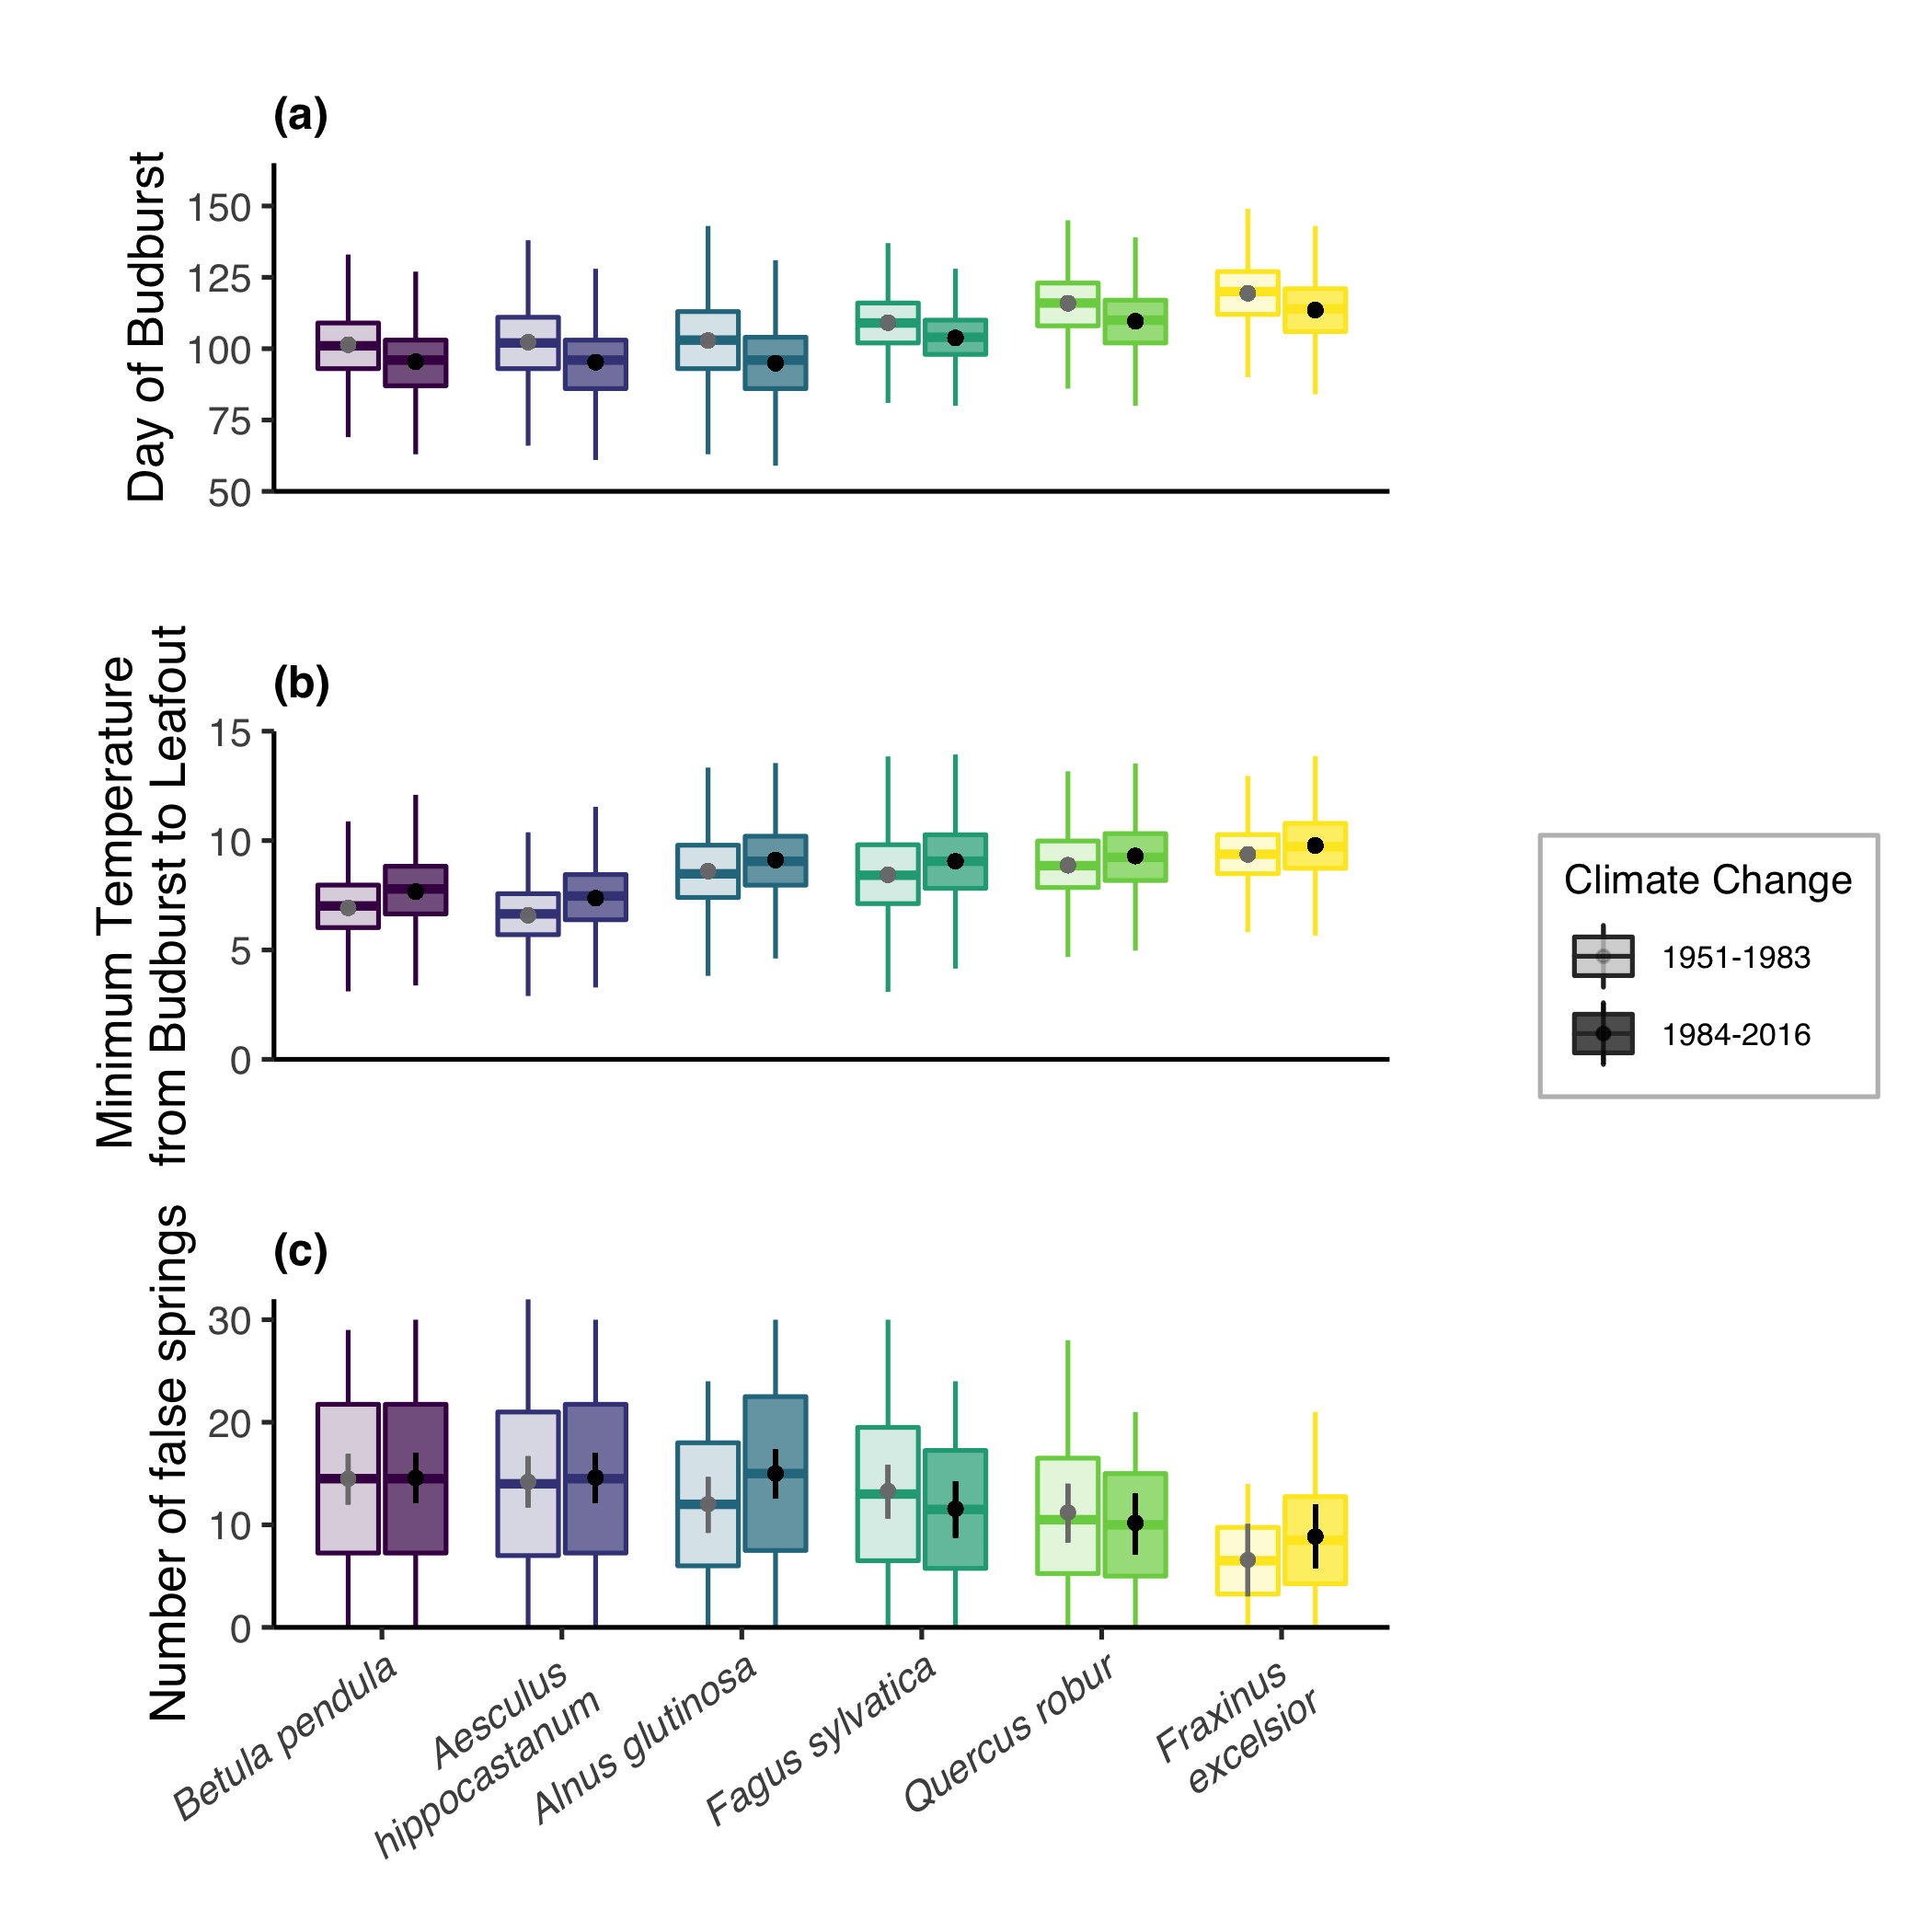
\includegraphics[width=14cm]{..//analyses/figures/Boxplot_BBTminFS_noDots_modestslong.png}
  -\caption{Day of budburst (\textbf{a}), minimum temperatures between budburst and leafout (\textbf{b}) and number of false springs (\textbf{c}) before and after 1983 across species for all sites. Box and whisker plots show the 25th and 75th percentiles (i.e., the interquartile range) with notches indicating 95\% uncertainty intervals. Dots and error bars overlaid on the box and whisker plots represent the model regression outputs (Tables \ref{tab:simbbmod}-\ref{tab:simpfs}). Error bars from the model regressions indicate 98\% uncertainty intervals but, given the number of sites, are quite small and thus not easily visible (see Tables \ref{tab:simbbmod}-\ref{tab:simpfs}). Species are ordered by day of budburst and are color-coded to match the other figures.  }\label{fig:boxfs}
  -\end{center}
  -\end{figure}}
  
  
{\begin{figure} [H]
  -\begin{center}
  %-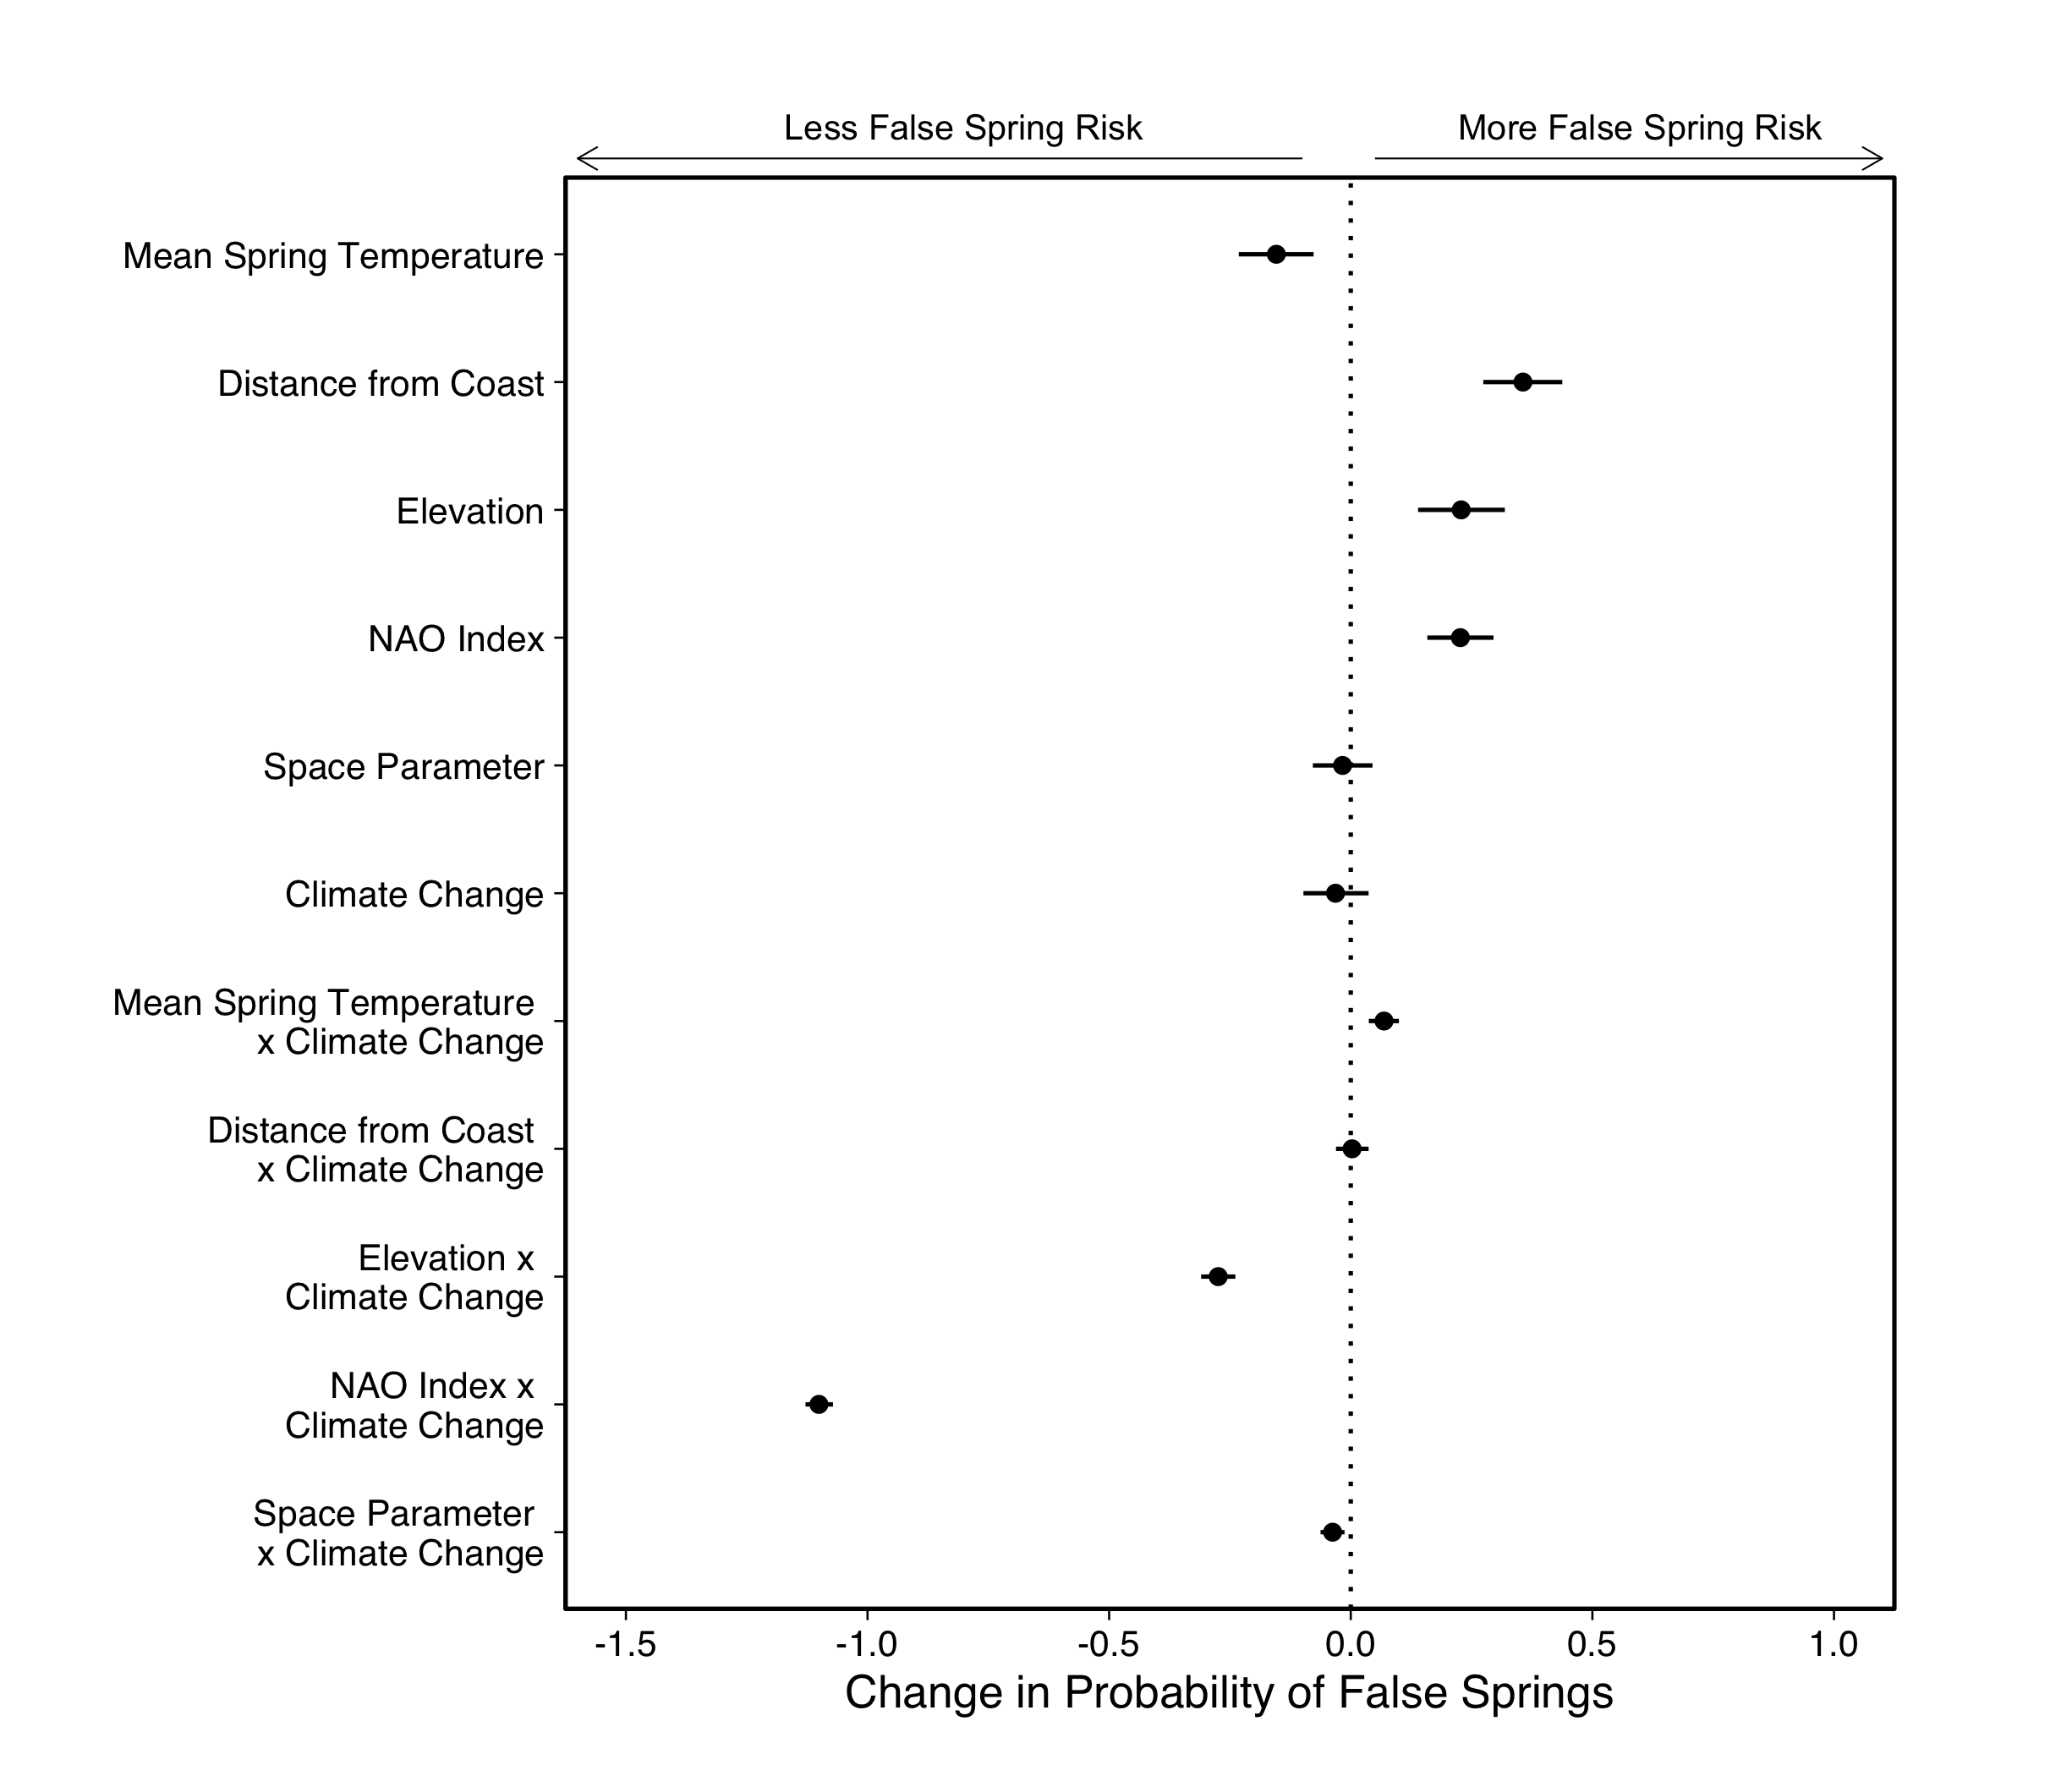
\includegraphics[width=12cm]{..//analyses/figures/model_output_98_long.png}
  -\caption{Effects of species, climatic and geographical predictors on false spring risk. More positive values indicate an increased probability of a false spring whereas more negative values suggest a lower probability of a false spring. Dots and lines show means and 98\% uncertainty intervals. There were 582,211 zeros and 172,877 ones for false springs in the data. See Table \ref{tab:suppmodlong} for full model output.}\label{fig:maineffects}
  -\end{center}
  -\end{figure}}

  
{\begin{figure} [H]
  -\begin{center}
  %-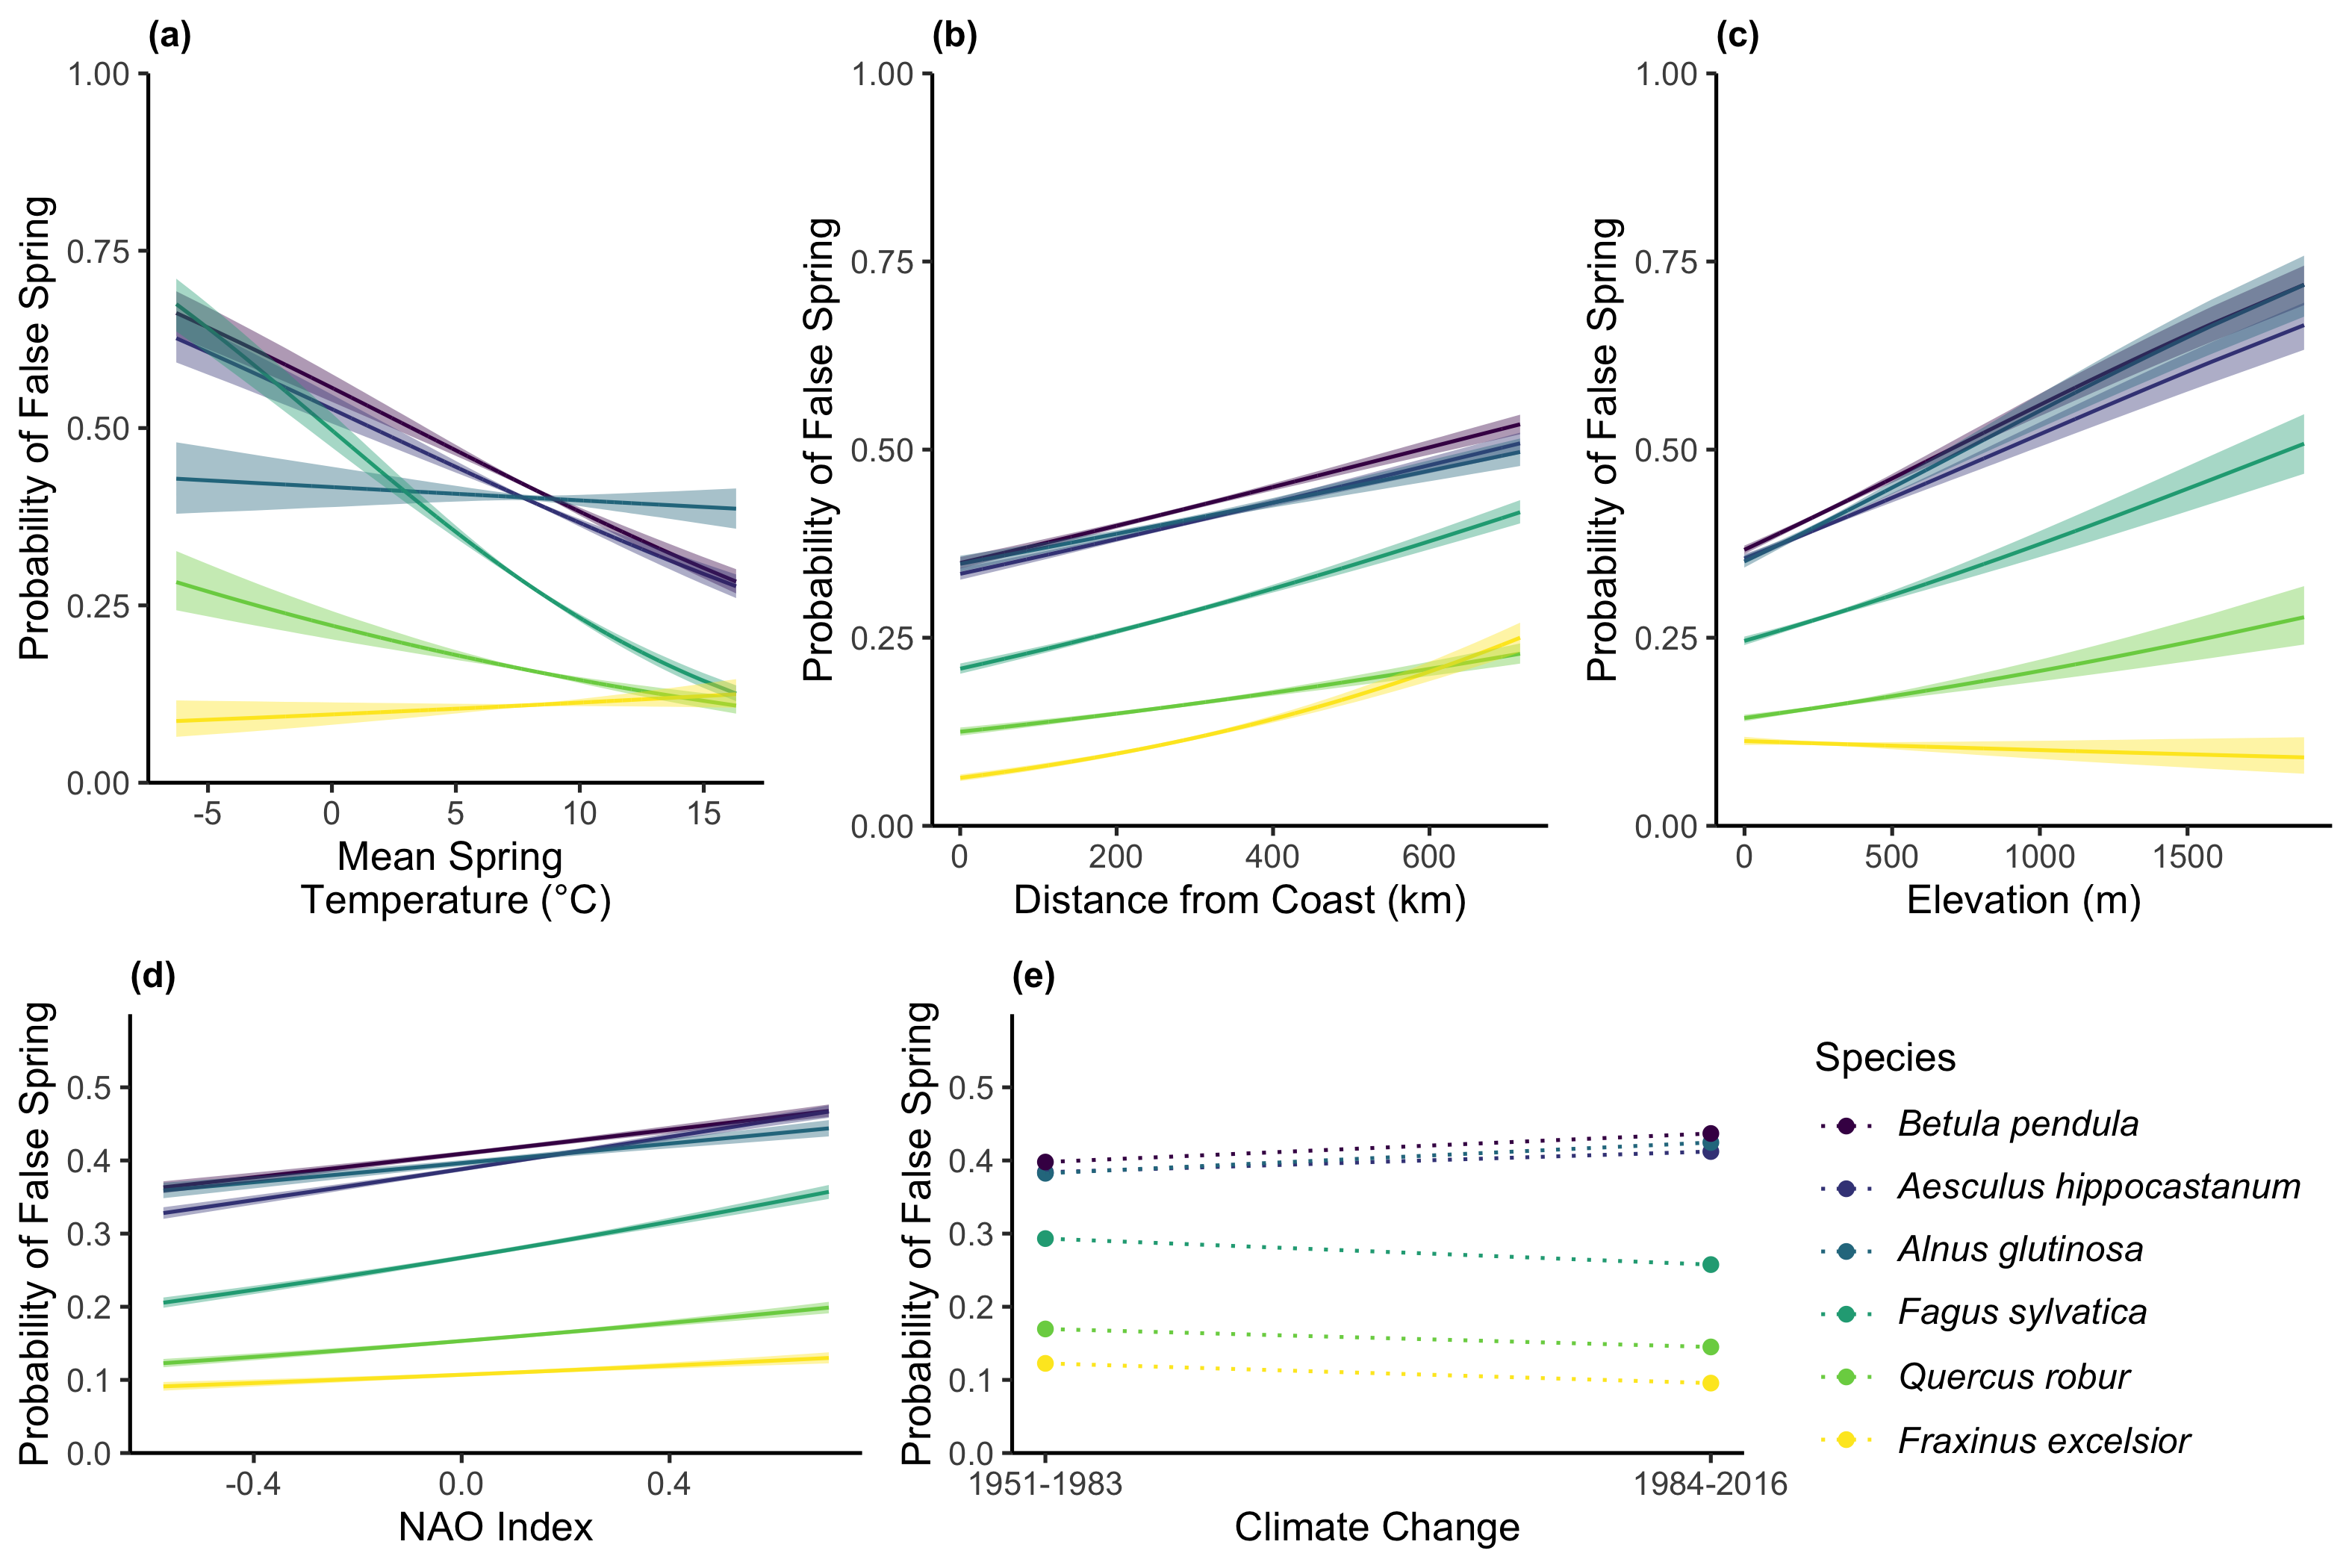
\includegraphics[width=16cm]{..//analyses/figures/InteractionPlots/Species_long.png}
  -\caption{Species-level variation across geographic and spatial predictors (i.e., mean spring temperature (\textbf{a}), distance from the coast (\textbf{b}), elevation (\textbf{c}), NAO index (\textbf{d})) and recent climate change (\textbf{e})). Lines and shading are the mean and 98\% uncertainty intervals for each species. To show results on the original scale of the data we converted model output. See Table \ref{tab:suppmodlong} for full model output. }\label{fig:spp}
  -\end{center}
  -\end{figure}}


  



\end{document}
